%!TEX TS-program = xelatex
%!TEX encoding = UTF-8 Unicode

\documentclass[12pt, a4paper]{article}

\usepackage{fontspec, xltxtra, xunicode}
\usepackage{amsfonts}
\usepackage{amssymb}
\usepackage{amsmath}
\usepackage{geometry}
\usepackage{clrscode3e}
% \geometry{left=1.25in, right=1.25in, top=1in, bottom=1in}

\usepackage{enumerate} % For listing things
\newfontfamily{\C}{STSongti-SC-Regular}
% \setlength\parindent{0pt}
\usepackage{listings}
\lstset{
  basicstyle=\footnotesize\ttfamily
}
\author{
  \begin{tabular}{c c c}
    QIU Yuheng {\C 邱渝桁} & YU Pengfei {\C 余鹏飞} & YU Xianggang {\C 余湘港} \\
    115010216              & 115010271              & 115010273
  \end{tabular}
}
\title {Course Project Report: Fast Template Matching}
\date{}
\begin{document}
\maketitle
\section{Problem Description}
  The problem focused in this project is that given a $K \times K$ template $T$, we need to find a patch in an $M \times N$ input image that is most similar to the given template. Therefore, we need to search for each possible patch in the $M \times N$ input image, and compare them with the given template. Eventually, we mark the best fit patch on the input image and return it.

\section{Algorithm}
  \subsection{Overview}
    We use totally 6 kernels and several CPU functions to complete the job.
    The job can be divided into the following parts: preprocessing, calculating
    the difference and finding the match.

    Our program also supports 2 features which are not stated in the
    Project Paper:
    \begin{enumerate}
      \item \textbf{Non-gray scale image} Details will be explained in the
            Reading Images (\ref{reading-image}) section.
      \item \textbf{Non-square templates} We modified the formulae in the Project
            Paper to support this feature, and detailed derivation will be in the
            Supporting Non-square Templates (\ref{non-square}) section.
    \end{enumerate}
  \subsection{Flowchart}
    Assuming maximal parallelism and ignore all the memory copying.

    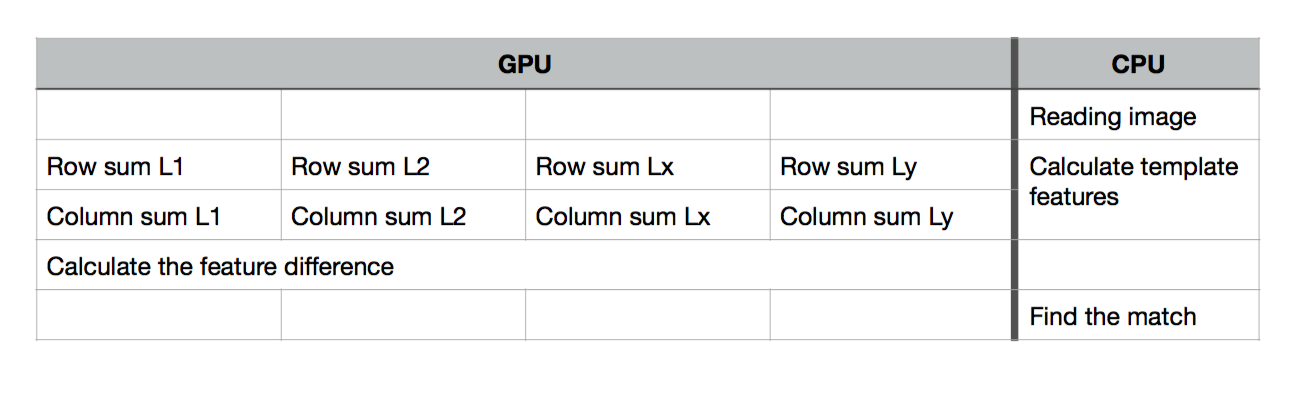
\includegraphics[scale=0.3]{flowchart.png}

  \subsection{Preprocessing}\label{preprocessing}
    \subsubsection{Reading Images}\label{reading-image}
      To support colorful (non-gray scale) images, we modify the BMP reading
      code:
      \begin{lstlisting}[language=c]
image[i * bmpwidth + j] = 0.11 * img_raw[i * linebyte + j * 3] +
                          0.59 * img_raw[i * linebyte + j * 3 + 1] +
                          0.30 * img_raw[i * linebyte + j * 3 + 2];
      \end{lstlisting}
      This code is to convert the colorful image to gray-scale by taking weighted
      average on RGB values of a pixel. And the formula is
      $I_{gray}=0.3I_R+0.59I_G+0.11I_B$. We assign a higher weight to green because
      green stimulates human's eyes more (BMP format stores a pixel in BGR order).
    \subsubsection{Calculate $L$ Tables}
      We use 5 kernels to calculate the $L$ tables of the 4 features. The first
      4 kernels calculate each row of the 4 tables respectively. And than the
      5th kernel will be launched 4 times on 4 different tables to sum up the
      tables by column. Because the code to sum up one table by column is the
      same for all 4 tables, we feed the 5th kernel with different row-summed
      table to calculate different $L$ table.
      We use CUDA streams to ensure that the 5th kernel only
      launches after the corresponding row-summed table is calculated. For example,
      the first stream will contain the first kernel (calcL1RowCumSum) that
      calculate first row-summed $L$ table (mean) and 5th kernel (calcSumTable).
      Thus the mean table will be summed up by column only after its rows are summed.

      For the grid and block size, we first use only 1 block with $M$ or $N$ threads
      in that block, where $M$ and $N$ are the dimension of the image. But this
      will fail if the image size is greater than $1024\times1024$. So our final
      method is to use $p$ threads in each block and let the total number of
      threads be about $M$ or $N$. The $p$ is the number of CUDA cores per SM,
      and we get this value at runtime. The reason for using this $p$ is that:
      threads in 1 block can only run on 1 SM and each SM can run at most $p$
      threads in the same time, so if we set the number of threads per block larger
      than $p$, the rest of threads will need to wait the first $p$ threads to
      finish. By setting each block $p$ threads, the blocks can be fully distributed
      on all SM and no thread needs to wait others (if there are enough cores).

      The formula of the grid size and block size is:
      \[\text{grid size: }\lfloor(M+p-1)/p\rfloor\text{ or }\lfloor(N+p-1)/p\rfloor\]
      \[\text{block size: }p\]

    \subsubsection{Calculate Template Features}
      As the template image is usually small, we use CPU to calculate the 4
      features of the template image by 1 loop. Also, we do not wait the GPU
      to finish before we calculate the template features by CPU. On the contrary,
      We overlap the computation of GPU and CPU, so hopefully we can reduce the
      time on waiting.

  \subsection{Calculating the Difference}
    The 6th kernel is used to calculate the difference between the feature vectors
    of the template and the patch. To ease the coding, we write a
    device function to calculate the $S$ value of a given patch from the $L$
    table. Then the calculation for the features of the patch and the square of
    Euclidean distance between 2 feature vectors is straightforward.

    The difference matrix is of size $(M-Kx+1)\times(N-Ky+1)$, so we need at least
    that number of threads to do the computation. However, if we use $N-Ky+1$
    threads per block, it is less efficient because this number may not be a
    multiple of 32. So we make the block size be $(32, p)$. Here $p$ is 16 if
    the GPU supports 512 thread per block and 32 if it supports 1024. And the
    final gird size and block size are:
    \[\text{grid size: }(\lfloor((M-Kx+1)+32-1)/32\rfloor, \lfloor((N-Ky+1)+p-1)/p\rfloor)\]
    \[\text{block size: }(32, p)\]
  \subsection{Finding the Match}
    We use CPU to find the minimal value and corresponding index in the difference
    matrix. It is just a sequential process: iterate through the whole matrix
    and find the minimum. The result index is just the bottom left corner of the
    matching patch.

  \subsection{Supporting Non-square Templates}\label{non-square}
    The only difference between square templates and non-square templates is how
    to calculate the feature vector. The formula of mean for the square templates
    is:
    \[v_1(D)=\frac{1}{K^2}S_1(D)\]
    The $K^2$ here means the area of $D$, so the formula of mean for the non-square
    template with size $K_x\times K_y$ is:
    \[v_1(D)=\frac{1}{K_xK_y}S_1(D)\]
    Similarly
    \[v_2(D)=\frac{1}{K_xK_y}S_2(D)-v_1(D)^2\]
    Things are little tricky for the gradients. From the original definition,
    the Extended Prewitt Operator on $x$ for the $K_x\times K_y$ patch is:
    \[EP_x(x, y)=x-\frac{K_x+1}{2}\]
    The absolute sum of $EP_x$ is:
    \[\sum_{i=1}^{K_x}\sum_{i=1}^{K_y}\left|EP_x(i,j)\right|\]
    \[=K_y\sum_{i=1}^{K_x}\left|EP_x(i,j)\right|\]
    \[=K_y\frac{(K_x+1)(K_x-1)}{4}\]
    So the gradient on $x$ is:
    \[G_x(D)=\sum_{i=1}^{K_x}\sum_{i=1}^{K_y}EP_x(i,j)I(i,j)/
      \sum_{i=1}^{K_x}\sum_{i=1}^{K_y}\left|EP_x(i,j)\right|\]
    \[=\sum_{i=1}^{K_x}\sum_{i=1}^{K_y}I(i,j)(x-\bar{x})/
      \sum_{i=1}^{K_x}\sum_{i=1}^{K_y}\left|EP_x(i,j)\right|\]
    where $x$ is the global index w.r.t. corresponding local index $i$ within the
    patch and $\bar{x}$ is the median of global index $x$ in this patch
    \[=\frac{4}{K_y(K_x+1)(K_x-1)}(S_x(D)-\bar{x}S_1(D))\]
    So similar as the formula (9) in the Project Paper, $v_3$ and $v_4$ can be
    written as:
    \[v_3(D)=\frac{4}{K_yK_x^2}(S_x(D)-xS_1(D))\]
    \[v_4(D)=\frac{4}{K_xK_y^2}(S_y(D)-yS_1(D))\]

\section{Analysis}
  \subsection{Preprocessing}
    At first, we use four kernels, and each kernel with $N$ threads, to compute the
    cumulative sum of mean value, variance, $X$ and $Y$ component of gradient on
    every row. Assuming the image size is $N \times N$, within each thread, there is
    a for loop with range $N$ to calculate the sum, so the time complexity of
    each thread is $O(N)$.

    Secondly, we launch 5th kernel four times to compute the cumulative sum on every column.
    Since we assume the image size is $N \times N$, so the 5th kernel also contains
    $N$ threads. And within each thread, there is also a for loop with range $N$ to
    calculate the sum, so the time complexity of each thread is $O(N)$.

    Thirdly, we use CPU to compute the template features. There are two for loops
    with range $K$ to complete the job, so the time complexity is $O(K^2)$.

    In conclusion, we launch kernel eight times, and each kernel has $N$ threads with
    time complexity $O(N)$. And we also use CPU to calculate template features, in which
    the time complexity is $O(K^2)$. So the time complexity of preprocessing is
    $8/64 \times N \times O(N) + O(K^2)$.
  \subsection{Calculating the Difference}
    We use one kernel with $(N - K + 1) \times (N - K + 1)$ threads to do the job.
    Within each thread, there is no loop, so the time complexity is $O(1)$, and the
    total time complexity of calculating the difference is $(N - K + 1) ^ 2 \times O(1)$ divided by 64.
  \subsection{Finding the Match}
    We use CPU to find the minimum among the difference vector. There are two for
    loops with range $N$ to search for the minimum, so the time complexity is $O(N ^ 2)$.
  \subsection{Conclusion}
    Since we divide the whole job into three parts, therefore the overall time complexity
    will be the sum of the time complexity of the above three parts. So the total
    time complexity is $8/64 \times N \times O(N) + O(K^2) + 1/64 \times O((N - K + 1) ^ 2) + O(N ^ 2)$.
    After simplification, the overall time complexity is $O(N ^ 2) + O(K ^ 2)$.


\section{Experiments}
  \subsection{Data}
  \subsection{Findings}

\section{Test Images}
  \begin{tabular}{|c|l|c|l|c|}
    \hline
    Image Name & Image Size       & Template Name & Template Size  & Color? \\\hline
    lena.bmp   & $512\times512$   & lena\_t.bmp   & $40\times40$   & No     \\\hline
    bridge.bmp & $612\times421$   & bridge\_t.bmp & $98\times58$   & Yes    \\\hline
    ll.bmp     & $3500\times2800$ & ll\_t.bmp     & $385\times265$ & Yes    \\\hline
    people.bmp & $1960\times1307$ & people\_t.bmp & $425\times613$ & Yes    \\\hline
    xu.bmp     & $1600\times1066$ & xu\_t.bmp     & $111\times115$ & Yes    \\\hline
  \end{tabular}

\section{Appendix and Vocabulary}
  \subsection{Project Paper}
    \textbf{Project Paper} refers to the pdf file ``project.pdf'' with title
    \textit{Course Project: Fast Template Matching}. In short, the guideline
    of this project.
  \subsection{Formula for Padding}
    You may see some formulae like $\lfloor(m+p-1)/p\rfloor$ in the report. This
    formula is used to calculate the minimal number of size $p$ boxes that can
    hold $m$ objects. A straightforward formula may be $\lfloor m/p\rfloor+1$,
    but this will give 1 more if $m$ is the multiple of $p$. For example, $m=100$
    and $p=10$.



\end{document}
